Antes de seguir con el desarrollo, es necesario explicar los estadísticos que se obtienen de realizar un entrenamiento con un modelo \texttt{YOLO}. En el caso de este trabajo, se realizará una 
explicación de los resultados que devuelve un modelo de detección.

Las métricas que se tienen en cuenta durante el entrenamiento son:

\begin{itemize}
    \item \textbf{Box Loss sobre el conjunto de entrenamiento}: representa el error del tamaño y posición de las \texttt{Bounding Boxes} de las etiquetas sobre las predichas en cada época. Cuando menor sea, 
    mayor es la cercanía entre las cajas predichas en el conjunto de entrenamiento respecto a sus etiquetas reales.\newline 
    Para calcularlo se utilizan métricas como la intersección entre unión, parámetro que indica cuanta parte del área coincide entre \texttt{bounding box} real y predicha. Su funcionamiento se puede observar 
    en la \autoref{fig:IoU}.

    \begin{figure}[H]
        \centering
        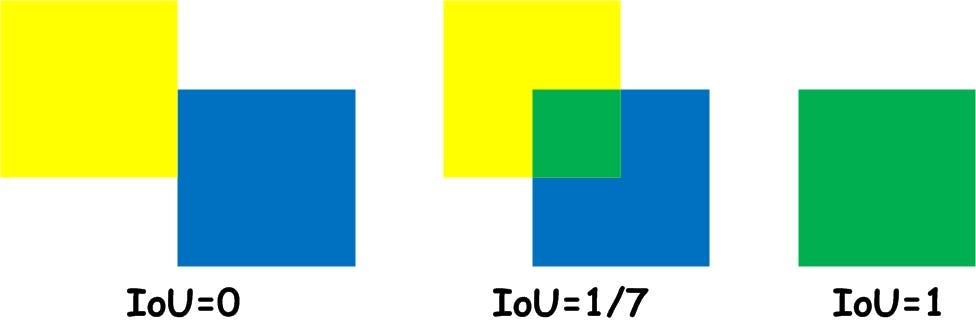
\includegraphics[width=0.4\textwidth]{images/13/a/IoU.png}
        \caption{Factor IoU para calcular la perdida de cajas en una \texttt{CNN} de detección}
        \label{fig:IoU}
    \end{figure}

    Aparte de esto, se utilizan otras métricas como la distancia, el ángulo de libertad respecto a la \texttt{bounding box} esperada y una medición de perdida en la relación alto/ancho de la caja.

    \item \textbf{Cls Loss sobre el conjunto de entrenamiento}: representa el error de clasificación de cada objeto detectado en la imagen respecto al de la etiqueta real en el conjunto de entrenamiento.
    \item \textbf{Dfl Loss sobre el conjunto de entrenamiento}: es un error sobre la capacidad del modelo \texttt{YOLO} para soportar deformaciones de los objetos detectados.
    \item \textbf{Precisión (B)}: indica la precisión general sobre los objetos detectados, para realizar este cálculo se tienen en cuenta todas las métricas anteriores como una media con pesos y condiciones. Idealmente es 1 como máximo.
    \item \textbf{Recall (B)}: indica la capacidad que se ha tenido para detectar todas las instancias, se utiliza después para saber cuantos elementos detecta con una precisión determinada. Idealmente es 1.
    \item \textbf{Métrica \acrshort{map}50 (B)}: es una métrica sobre la precisión media en elementos con una intersección entre unión de \texttt{0.5}. Esta métrica se puede entender como la capacidad de detección 
    en elementos fáciles de forma correcta. Es bastante representativa en el entrenamiento para saber si algo malo esta sucediendo.
    \item \textbf{Métrica \acrshort{map}50-95 (B)}: igual que antes, representa una media ponderada de precisión, pero en este caso de los elementos con una intersección entre unión en el rango de \texttt{0.5} a 
    \texttt{0.95}. Podemos considerar esto como las detecciones dificiles y ajustadas a los resultados que esperamos.
    \item \textbf{Box Loss sobre el conjunto de validación}: igual que el \texttt{Box Loss} sobre el conjunto de entrenamiento, pero en este caso, al no variar el conjunto de validación, se va tomando como referencia 
    entre épocas para saber si el entrenamiento esta siendo correcto.
    \item \textbf{Cls Loss sobre el conjunto de validación}: igual que en la situación de entrenamiento pero como métrica entre épocas en un conjunto de datos invariante.
    \item \textbf{Dfl Loss sobre el conjunto de validación}: igual que en la situación de entrenamiento pero como métrica entre épocas en un conjunto de datos invariante para la precisión en deformación.
\end{itemize}

Estas métricas idealmente van acercándose a valores aceptables según pasan las épocas. Esto puede ser guardado al finalizar un entrenamiento de forma automática por parte de \texttt{YOLO} como se puede ver en el 
ejemplo de la \autoref{fig:ResultadosEjemplo} para 100 épocas.

\begin{figure}[H]
    \centering
    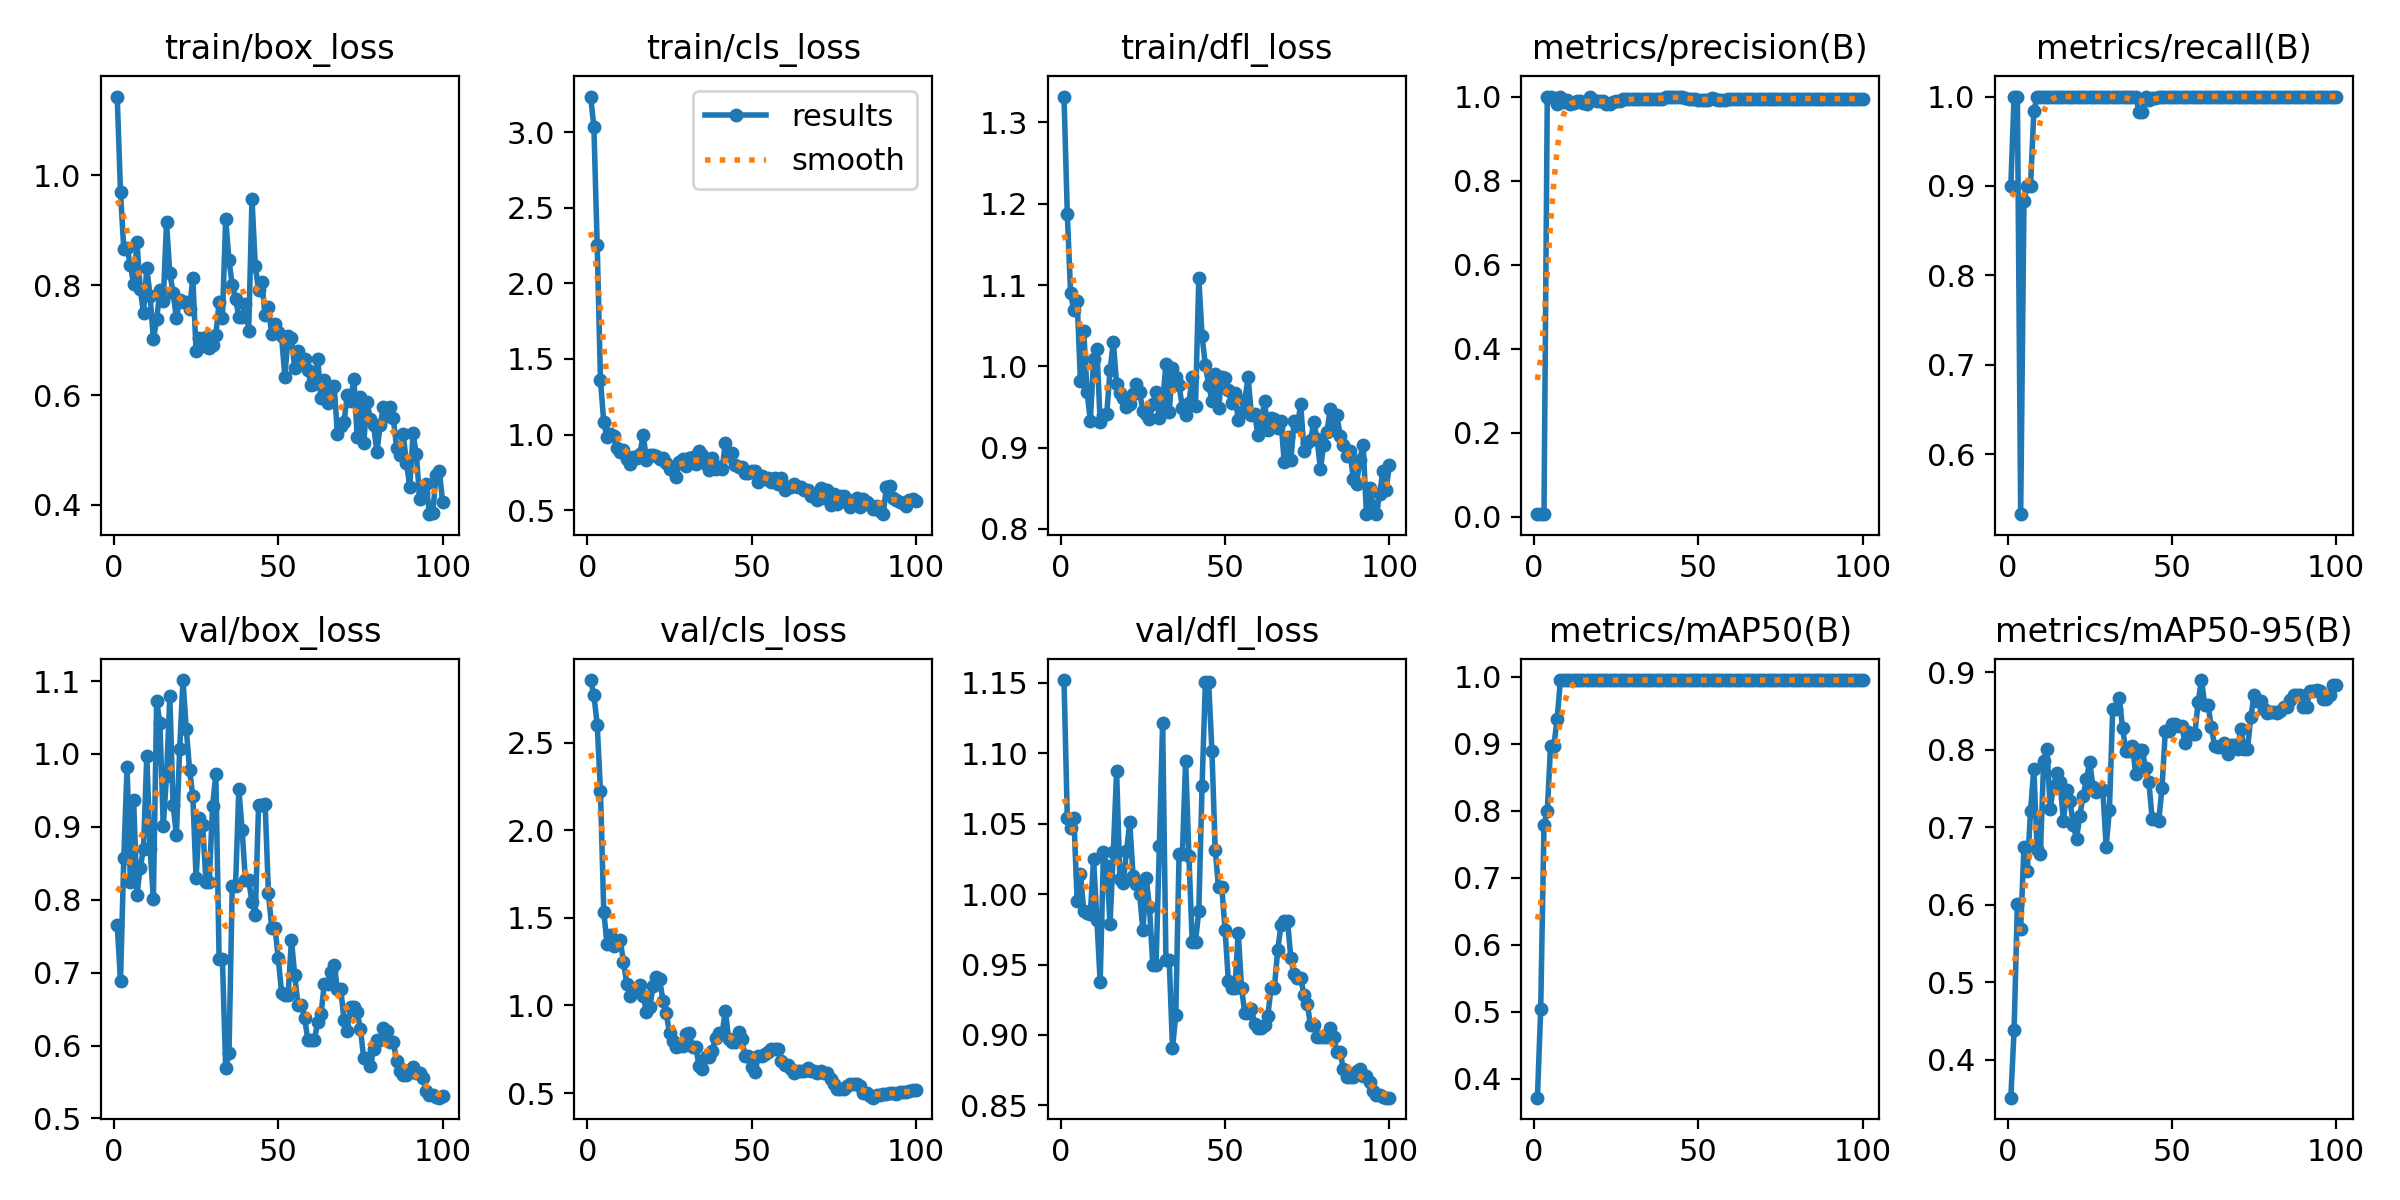
\includegraphics[width=0.95\textwidth]{images/13/a/results.png}
    \caption{Ejemplo de imagen de resultados resumidos por parte de \texttt{YOLO}}
    \label{fig:ResultadosEjemplo}
\end{figure}
\clearpage
Adicionalmente, \texttt{YOLO} produce resultados adicionales, que dependiendo del objetivo de la red, se buscará maximizar uno u otro:

\begin{itemize}
    \item \textbf{Matriz de confusión}: es una matriz como la de la \autoref{fig:MatrizEjemplo},que muestra el número de objetos detectados y su clasificación, si el objeto está correctamente clasificado será un verdadero positivo, si 
    se piensa que hay objeto, pero no hay, será falso positivo y si no se detecta, pero existe será falso negativo. Finalmente se tiene la situación de un verdadero negativo si no hay y no se detecta un objeto. Al ser un 
    estadístico de clasificación por naturaleza, no es el más apropiado para el análisis de resultados en detección de objetos, y menos cuando solo hay 1 clase de objetos.

    \begin{figure}[H]
        \centering
        \includegraphics[width=0.35\textwidth]{images/13/a/MatrizConfusiónEjemplo.png}
        \caption{Ejemplo de matriz de confusión en la medicina}
        \label{fig:MatrizEjemplo}
    \end{figure}

    \item \textbf{Curva de puntuación F1}: representa la puntuación F1, que se calcula a través de \begin{equation*}\text{Puntuación F1} = \frac{2*Precision*Recall}{Precision+Recall}\end{equation*} siendo el recall 
    calculado como: \begin{equation*}\text{Recall} = \frac{TP}{TP+FN}\end{equation*} Cuanto mayor área tenga bajo la curva mejor, porque significará que hay más verdaderos positivos en precisiones altas respecto a falsos.
    \item \textbf{Curva de precisión contra recall}: muestra la relación entre precisión y recall, mostrando una relación entre los valores seleccionados para seleccionar umbrales.
    \item \textbf{Curva de precisión}: refleja para cada valor de confianza de clasificación de elemento la precisión media de esa asignación. Cuanto más plana y cercana al 1 sea, mejor. Idealmente sería un escalón.
    \item \textbf{Curva de recall}: muestra para cada valor de confianza, el recall medio en ese valor. Idealmente es una línea horizontal en \texttt{y=1}.
\end{itemize}
